\chapter{L'implementazione}
In questo capitolo verranno illustrati i framework utilizzati per l'implementazione dell'applicazione e l'algoritmo ideato per la creazione di una griglia sulla mappa con il relativo codice Javascript.
\section{Le applicazioni cross-platform}
Negli ultimi anni, i dispositivi mobili sono diventati sempre più parte integrante della nostra vita, grazie al progresso tecnologico e all'abbattimento dei prezzi, oggi costituiscono un bene alla portata di tutti. \\
La possibilità di scegliere tra una vasta gamma di smartphone diversi per caratteristiche e produttore, ha reso più complicata la vita delle aziende informatiche che sono costrette a considerare l'eterogeneità dei vari sistemi operativi in circolazione.\\
\begin{figure}[H]
	\centering
	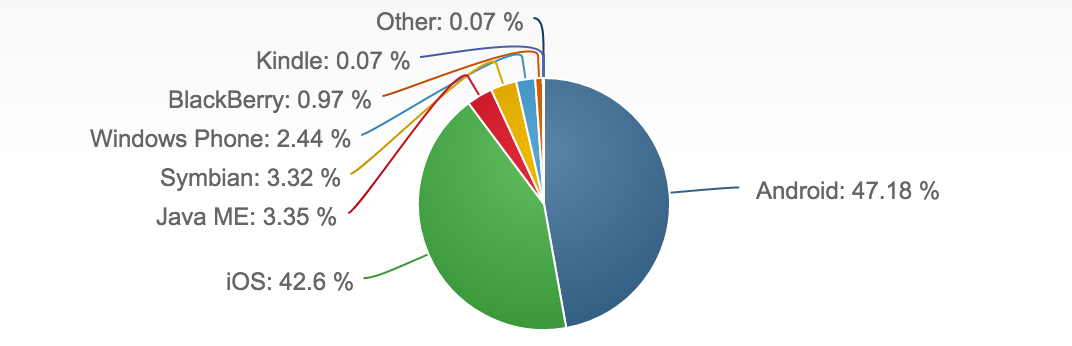
\includegraphics[scale=0.7]{Implementazione/os.png}
	\caption{Utilizzo dei vari OS su scala mondiale}
	\label{fig:os_mobile}
\end{figure}
\newpage
Chi sviluppa applicazioni mobili, può scegliere tra due approcci:
\begin{enumerate}
\item \textbf{Scegliere uno degli OS mobile} e implementare l'applicazione utilizzando il linguaggio nativo.
\item \textbf{Scegliere un framework }che, utilizzando un meta-linguaggio, sia in grado di generare diverse versioni dell'applicazione per i relativi OS.
\end{enumerate}
I diversi approcci forniscono rispettivamente pro e contro. Per il primo i vantaggi sono una maggiore velocità del sistema, la possibilità di creare un'interfaccia rispettando il look and feel nativo e pochi problemi di compatibilità. Lo svantaggio è invece legato alla \textbf{bassa portabilità}, l'applicazione andrà riscritta completamente per dispositivi con diversi OS. \\
Il principale vantaggio del secondo approccio, è invece la possibilità di riutilizzare lo stesso codice per generare varie versioni dell'applicazione per diversi OS, questo a discapito di una minore velocità del sistema se l'applicazione fosse sviluppata nel linguaggio nativo. \\
Considerando il contesto d'uso del sistema ( vedi \ref{contesto}), è chiaro che la nostra applicazione dovrebbe poter essere installata su qualsiasi dispositivo (ndr l'idea di salvare vite con un certo OS non è delle più nobili), di conseguenza si è adottato tale approccio.\\
La filosofia \textit{"Write once, run anywhere"}, non è un concetto nuovo nell'informatica, lo slogan fu ideato dalla Sun Microsystems per descrivere un linguaggio (Java) in grado di essere eseguito su diverse macchine. Nel corso degli anni diverse software-house hanno realizzato dei framework in grado di fare questa "magia", sostanzialmente ne estitono due tipi:
\begin{itemize}
\item \textbf{ I Cross-Compiling:} si scrive l'applicazione in un certo linguaggio, successivamente un framework riesce a compilarlo per le diverse piattaforme (Appcelerator Titanium1, Corona SDK2, Xamarin Monotouch3); Solitamente sono framework professionali e a pagamento.
\item \textbf{I Browser-Embedding:} più recenti, consentono di sviluppare il codice con le tecnologie del web (HTML5, CSS3, Javascript), l'applicazione verrà avviata nel dispositivo mobile all'interno di un browser (PhoneGap, Apache Cordova).
\end{itemize} 
Ancora una volta è stato scelto il secondo approccio, nello specifico il framework PhoneGap.

\section{PhoneGap}
\label{phonegap}
Phonegap è un framework di sviluppo mobile prodotto da Nitobi e acquistato successivamente da Adobe Systems. Permette ai programmatori software di creare applicazioni per dispositivi mobili utilizzando esclusivamente HMTL, CSS e Javascript invece di utilizzare linguaggi nativi come Object-C e C++. Il risultato sono applicazioni ibride, nel senso che non sono né del tutto native (perché tutto il rendering del layout è fatto tramite viste web e non tramite i framework UI delle piattaforme native) né del tutto web-application (perché non sono applicazioni solo web, ma hanno anche accesso alle funzioni interne dei device tramite le API). \\
Il software alla base di PhoneGap è \textit{Apache Cordova} ed è open source. \\
\begin{figure}[H]
	\centering
	
\includegraphics[scale=0.6]{Implementazione/logo_phonegap.png}
	\caption{Logo del framework PhoneGap}
	\label{fig:logo_phonegap}
\end{figure}
Presentato la prima volta in un evento iPhoneDevCamp a San Francisco, PhoneGap ha vinto il premio People's Choice Award alla conferenza O'Reilly Media Web nel 2009. Il framewotk PhoneGap viene utilizzato da molte piattaforme  di sviluppo software come ViziApps, Worklight, Convertico e appMobi. \\
Il 4 ottobre 2011 Adobe annuncia ufficialmente l'acquisizione della Nitobi Software. In concomitanza il codice PhoneGap ha contribuito con la Apache Software Foundation ad iniziare un nuovo preocetto chiamato Apache Cordova.
\newpage
PhoneGap non è altro che un modulo software che permette agli sviluppatori di incorporare le loro applicazioni web all'interno di applicazioni native di diverse piattaforme. Le applicazioni che utilizzano questo framework sono scritte in HTML5, CSS3 e Javascript e il collegamento con le livrerie native, specifiche di ogni piattaforma, è fatto tramite le API che mette a disposizione il framework.
PhoneGap fa quindi da ponte tra il sistema operativo e la web application realizzata dallo sviluppatore. Indipndentemente dalla piattaforma sottostante esisterà un modo per invocare le API native mediante funzioni Javascript. \\
Il programmatore quindi utilizzerà le API fornite da PhoneGap per accedere alle risorse hardware e software del device in modo da aggiungere le funzionalità di base al motore JAvascript e renderle facilmente utilizzabili come se fossere vere e propri metodi di una libreria. Dopo la compilazione, che avviene tramite il servizio cloud \textbf{PhoneGap Build} (Figura \ref{fig:phonegap_build}), viene generato un pacchetto internamente composto da due elementi principali con differenti responsabilità che però cooperano tra loro per fornire delle funzioni a valore aggiunto. In pratica esiste un runtime basato su WebKit4 in cui vengono iniettate le componenti statiche; il risultato sarà un pacchetto composta da due elementi principali con differenti responsabilità che però cooperano tra loro per fornire delle funzioni a valore aggiunto. Nel caso specifico il runtime si occupa di dialogare direttamente con il dispositivo e le parti statiche offrono l'interfaccia verso l'utente. L'uso di Javascript e Ajax consente poi di rendere le applciazioni più complesse e dinamiche.
\begin{figure}[H]
	\centering
	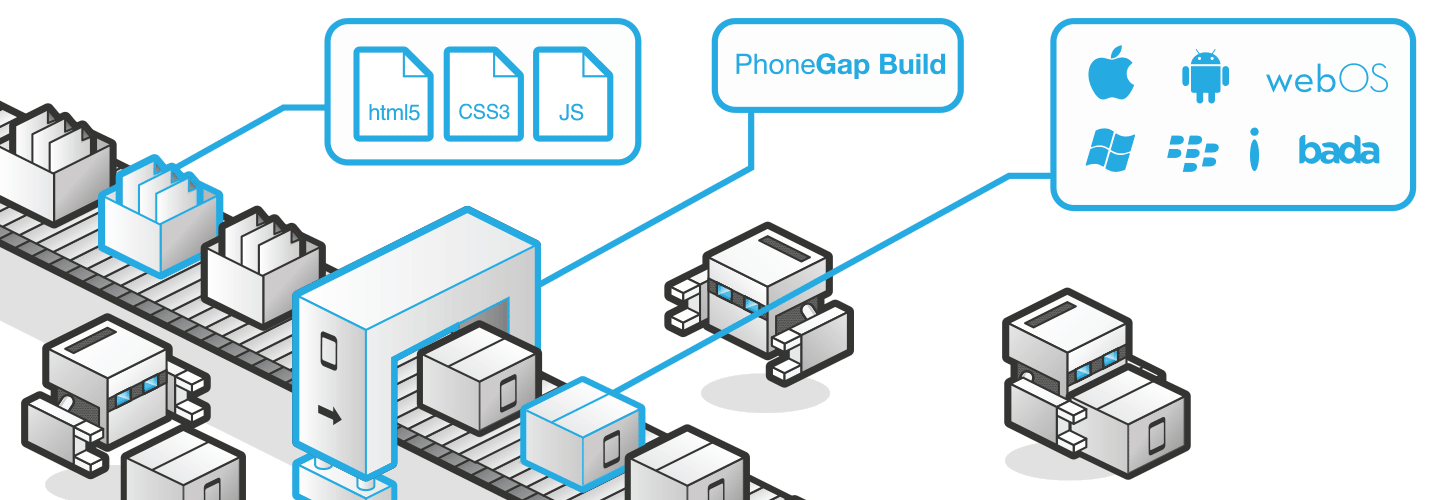
\includegraphics[scale=0.3]{Implementazione/phonegap_build.png}
	\caption{Logo del framework PhoneGap}
	\label{fig:phonegap_build}
\end{figure}

\newpage
Ora illustriamo mediante la Figura \ref{fig:architettura_phonegap} come è strutturata l'architettura PhoneGap. Partendo dal basso verso l'alto, si può notare che la parte in blu è quella del sistema operativo della piattaforma nativa che si trova sui vari device. Al livello immediatamente successivo troviamo il framework PhoneGap (in grigio) che ci viene fornito insieme alle API Javascript. Da notare il rettangolo arancione che rappresenta l'embedded browser che incapsula la web application e le API. Di default il browser viene aperto esternamente all'applicazione. Di conseguenza ad ogni richiesta di una pagina web avviene l'apertura di un bottone fornito dal browser. In pratica si rende impossibile notare che si tratta di un browser e quindi di una pagina web. Ciò rende l'applicazione più simile ad un applicazione nativa.\\
Infine, in verde è evidenziata la parte a carico dello sviluppatore che è la vera e propria web application, realizzata all'interno del framework PhoneGap.
\begin{figure}[H]
	\centering
	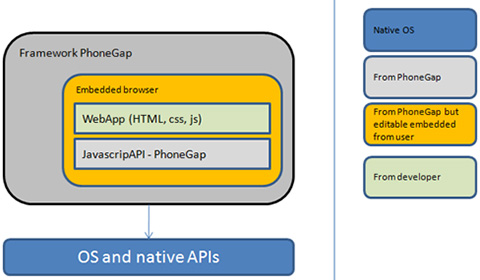
\includegraphics[scale=0.9]{Implementazione/phonegap_architettura.jpg}
	\caption{Architettura di un'applicazione realizzata con PhoneGap}
	\label{fig:architettura_phonegap}
\end{figure}

Come detto PhoneGap mette a disposizione del programmatore, una serie di API per l'accesso all'hardware nativo del device. Bisogna tenere conto però che non tutte le piattaforme hanno a disposizione gli stessi sensori e che occorre prestare molta attenzione nel caso in cui il building dell'applicazione è fatto su piattaforme diverse. Il framework, infatti, offre supporto per ogni piattaforma degna di essere presa in considerazione ovvero: Android, iOS, Symbian, WebOS, Blackberry etc. Non tutte le piattaforme son però supportate allo stesso modo. La seguente tabella (Fig \ref{fig:tabella_api} )
riassume lo stato dell'arte riguardo la compatibilità e l'accessibilità che il framework offre verso i sensori presenti nei diversi device, equipaggiati da diversi OS.

\begin{figure}[H]
	\centering
	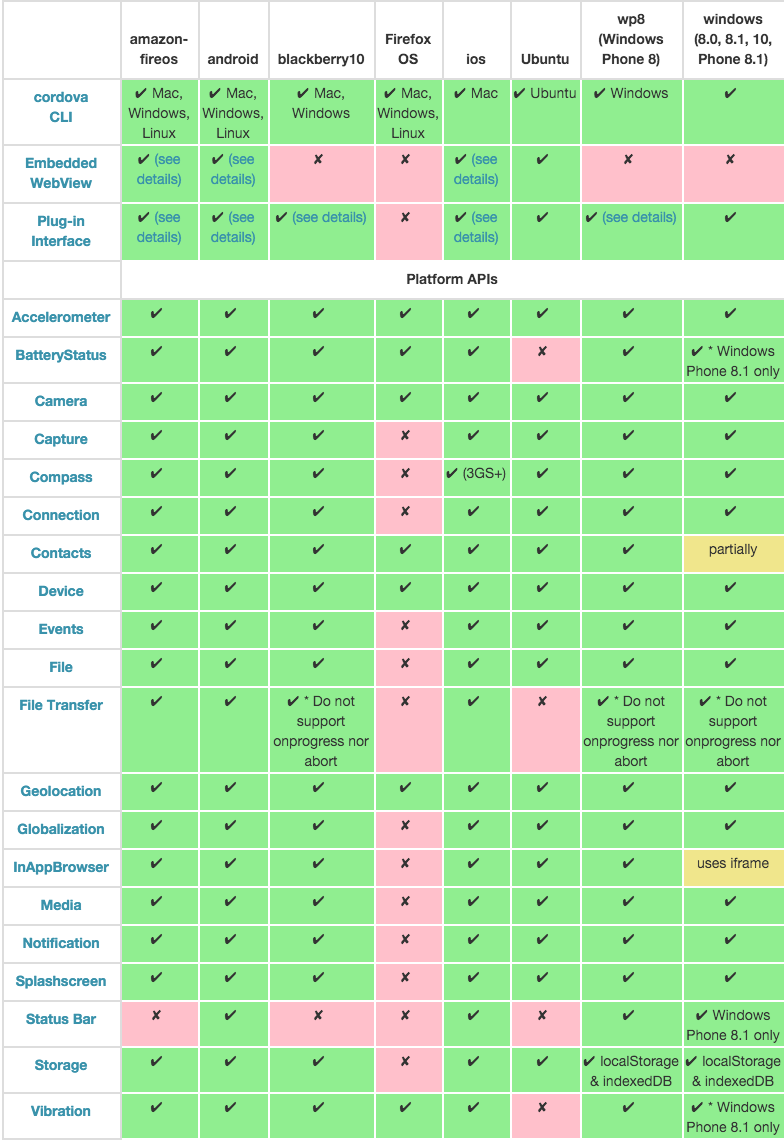
\includegraphics[scale=0.8]{Implementazione/phonegap_api.png}
	\caption{Le API e il loro supporto per le varie piattaforme}
	\label{fig:tabella_api}
\end{figure}

\section{Ratchet}
\label{ratchet}
Il solo utilizzo del framework PhoneGap non è sufficiente per realizzare un'applicazione degna di nota. L'interfaccia grafica costituisce un'elemento fondamentale nelle moderne applicazioni mobili. Inoltre, se ben progettata, contribuisce ad aumentare la user experience \cite{EXPERIENCE} e in generale l'usabilità del sistema stesso. A tale proposito è stato utilizzato il framework opens source \textbf{Ratchet} [http://goratchet.com/].

\begin{figure}[H]
	\centering
	
\includegraphics[scale=1]{Implementazione/ratchet_logo.png}
	\caption{Il logo del framework Ratchet}
	\label{fig:logo_ratchet}
\end{figure}

I componenti grafici offerti da questo strumento sono responsive e appositamente progettati per gli smartphone; il loro utilizzo è tanto semplice quanto efficace, analogamente ad altri progetti di successo, come Bootstrap, i componenti possono essere inclusi nell'interfaccia aggiungendo dello specifico codice HTML e vari stili CSS (costumizzabili a proprio piacimento). A partire dalla seconda versione è stata integrata una classe di icone con immagini di uso comune nelle applicazioni mobili.\\
La combinazione di questo tool insieme ad altri per l'accesso al DOM (Document Object Model) dell'applicazione (vedi \ref{phonegap}), nel nostro caso \textit{jQuery}, permette di realizzare applicazioni con un'interfaccia accattivante e molto simile a quelle native.
\newpage
Ad esempio per aggiungere la "classica" tab-bar basta inserire il seguente codice HTML:
\begin{lstlisting} [language=XML]
<nav class="bar bar-tab">
  <a class="tab-item active" href="#">
    <span class="icon icon-home"></span>
    <span class="tab-label">Home</span>
  </a>
  <a class="tab-item" href="#">
    <span class="icon icon-person"></span>
    <span class="tab-label">Profile</span>
  </a>
  <a class="tab-item" href="#">
    <span class="icon icon-star-filled"></span>
    <span class="tab-label">Favorites</span>
  </a>
  <a class="tab-item" href="#">
    <span class="icon icon-search"></span>
    <span class="tab-label">Search</span>
  </a>
  <a class="tab-item" href="#">
    <span class="icon icon-gear"></span>
    <span class="tab-label">Settings</span>
  </a>
</nav>
\end{lstlisting}
\newpage
Ed ottenere il seguente risultato:
\begin{figure}[H]
	\centering
	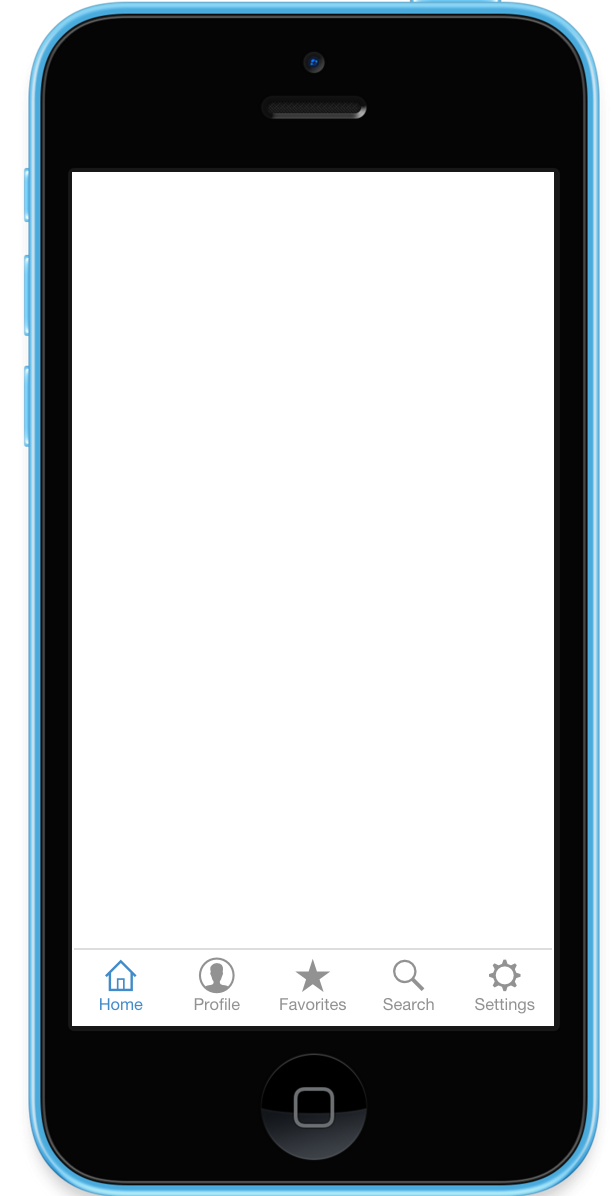
\includegraphics[scale=0.7]{Implementazione/tab-bar.png}
	\caption{Il componente tab-bar con cinque icone}
	\label{fig:tab}
\end{figure}

\newpage
\section{Leaflet}

Per la mappa interattiva si è utilizzata la libreria \textbf{ Leaflet} \cite{LEAFLET}. Leaflet è una libreria open source JavaScript per le mappe interattive mobili-friendly. Con nn peso di soli circa 33 KB di JS, ha tutte le caratteristiche e le maggiori funzioni necessarie agli sviluppatori.\\
Leaflet è stato progettato per avere alte prestazioni ed facilmente utilizzabile. Funziona in modo efficiente su tutte le principali piattaforme desktop e mobile, può essere estesa con un sacco di plugin e la documentazione è ben fatta.\\

\begin{figure}[H]
	\centering
	
\includegraphics[scale=0.5]{Implementazione/leaflet.png}
	\caption{Il logo della libreria Leaflet}
	\label{fig:leaflet}
\end{figure}

Il codice per inserire una mappa all'interno di un \textit{div} con \textit{id='map'} è semplicemente:
\begin{lstlisting} [language=JavaScript]
var map = L.map('map').setView([51.505, -0.09], 13);

L.tileLayer('http://{s}.tile.osm.org/{z}/{x}/{y}.png', {
    attribution: '&copy; <a href="http://osm.org/copyright">OpenStreetMap</a> contributors'
}).addTo(map);
//aggiunge un marker alle coordinate [51.5,-0.09]
L.marker([51.5, -0.09]).addTo(map)
    .bindPopup('A pretty CSS3 popup.<br> Easily customizable.')
    .openPopup();
\end{lstlisting}
Con il seguente risultato:
\begin{figure}[H]
	\centering
	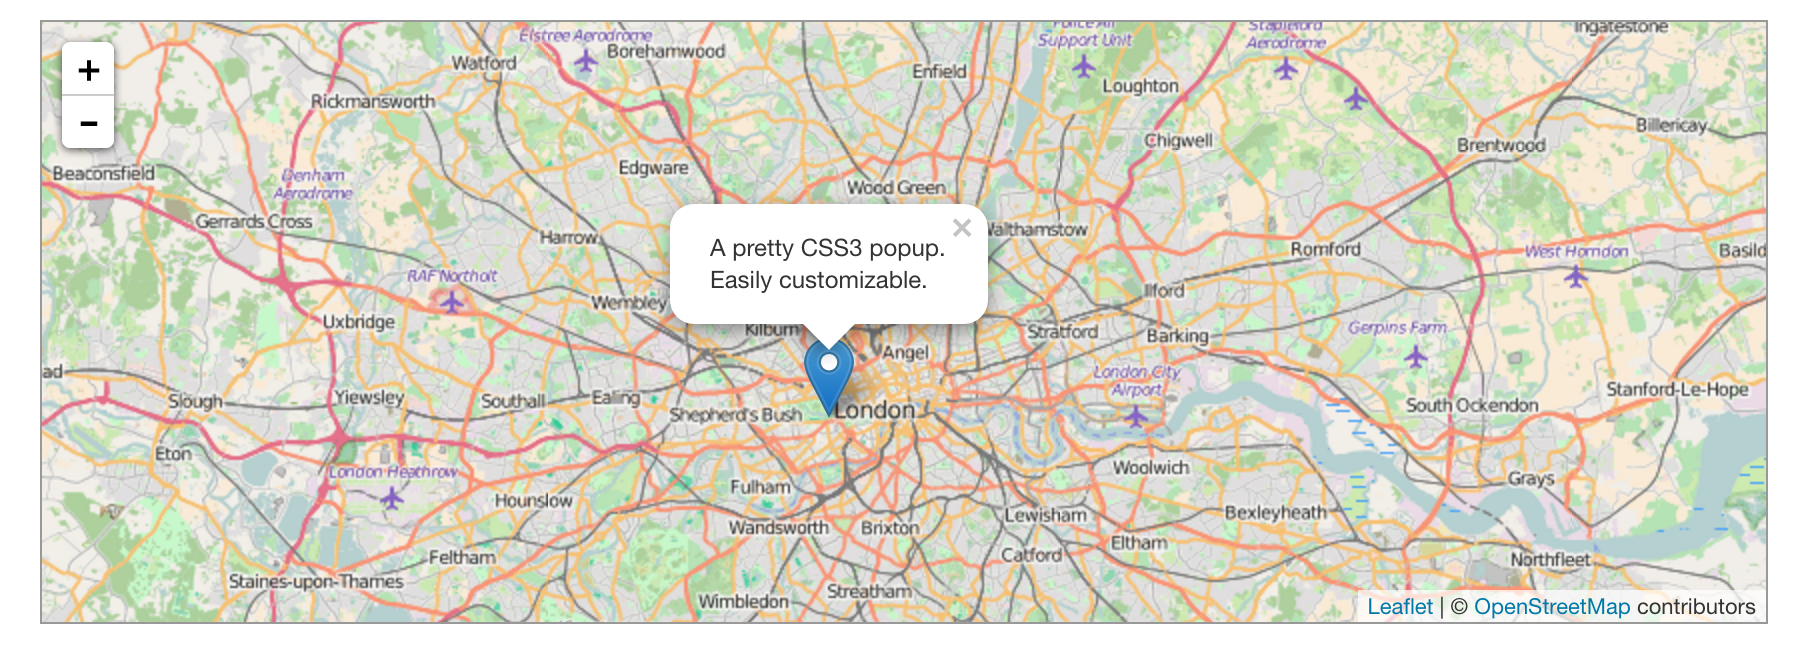
\includegraphics[scale=0.4]{Implementazione/leaflet_result.png}
	\caption{Risultato grafico con il codice precedente}
	\label{fig:leaflet_result}
\end{figure}
Le coordinate sono implementate attraverso l'oggetto latLng, ed è possibile crearne delle nuove nel seguente modo:
\begin{lstlisting} [language=JavaScript]
var latlng = L.latLng(50.5, 30.5);
\end{lstlisting}
Come detto la libreria dispone di una grande quantità di funzioni e metodi utili, ad esempio l'evento sulla geolocalizzazione:
\begin{lstlisting} [language=JavaScript]
	function onLocationFound(e) {
	console.log("localizzato!!")
};
\end{lstlisting}
L'oggetto \textit{"e"} contiene al suo interno, oltre alle coordinate, altri oggetti utili come la velocità, l'orario, l'altitudine ect.\\
Esistono altre librerie per utilizzare i dati ottenuti da un server OpenStreetMap, tuttavia questa si è rivelata essere molto efficente e semplice; merito di una curva di apprendimento buona e della ricca e chiara documentazione fornita. Inoltre è stato utilizzato un plugin che permette di salvare, in locale al device, la mappa visualizzata dall'utente su diversi livelli di zoom.

\newpage
\section{La griglia trasparente}
Come specificato nei requisiti di sistema, l'utente e gli eventi devono essere associati in modo univoco ad una cella di grandezza $(22*16)mt^{2}$; per fare ciò è necessario che il sistema sia in grado di "costruire" dinamicamente una griglia. Questa deve essere del tutto invisibile agli utenti che non hanno alcun interesse a conoscere o comprendere tale dettaglio implementativo.\\
Prima di spiegare la soluzione a questo problema occorre fare un passo indietro, sin dai tempi più remoti l'uomo ha cercato di creare delle mappe cartografiche. Le più antiche testimonianze \cite{GROTTE} conosciute di qualcosa che assomigli ad una rappresentazione cartografica non riguardano la terra, ma il cielo, così come appare di notte. Sui muri delle grotte di Lascaux sono stati infatti osservati dei puntini dipinti databili al 16.500 a.C. che rappresentano il cielo notturno ed in cui si possono riconoscere Vega, Deneb e Altair (il cosiddetto Triangolo estivo), nonché le Pleiadi. Da allora la cartografia ha fatto passi da gigante(vedi cap \ref{cap:OpenStreetMap}).\\
Tornando al nostro problema, la soluzione trovata si basa sul calcolo della distranza tra due coordinate geografiche, il cui problema è il calcolo stesso. Non avendo la Terra una forma lineare, è difficile trovare una rappresentazione geometrica perfetta di essa. \\
Gli algoritmi più utilizzati per il calcolo della distanza tra due punti, utilizzano le formule di Haversine e Vincenty, il primo si basa sull'approssimazione della terra ad una sfera perfetta, mentre il secondo la modelizza in uno sferoide oblato. \\
E' bene dire che mentre il risultato ottenuto tramite la formula di Haversine può avere un'errore dello 0,3\%  quello di Vincenty è molto più accurato, con un errore di 0.5mm circa; questa precisione si ha a discapito di un costo computazionale più elevato. Per brevi distanze i metodi tendono invece a convergere.
\newpage
\subsection{L'algoritmo Santiago}
\label{santiago}
Con entrambi gli algoritmi è stato verificato che una variazione unitaria di $10^{-4} $ gradi in latitudine corrisponde ad una distanza di 11 mt, 8 mt se in longitudine. Partendo da questo risultato si è così ideato il seguente algoritmo.

\begin{enumerate}
\item Per prima cosa, si considera l'utente posto all'interno di un sistema di riferimento calcolato troncando le sue coordinate alla terza cifra decimale. La grandezza fisica di questi sistemi è quindi di $ 9680mt^{2} $. L'origine corrisponde alle coordinate dell'utente troncate alla $10^{-4} $, con l'ultima cifra decimale uguale a zero.
\begin{figure}[H]
	\centering
	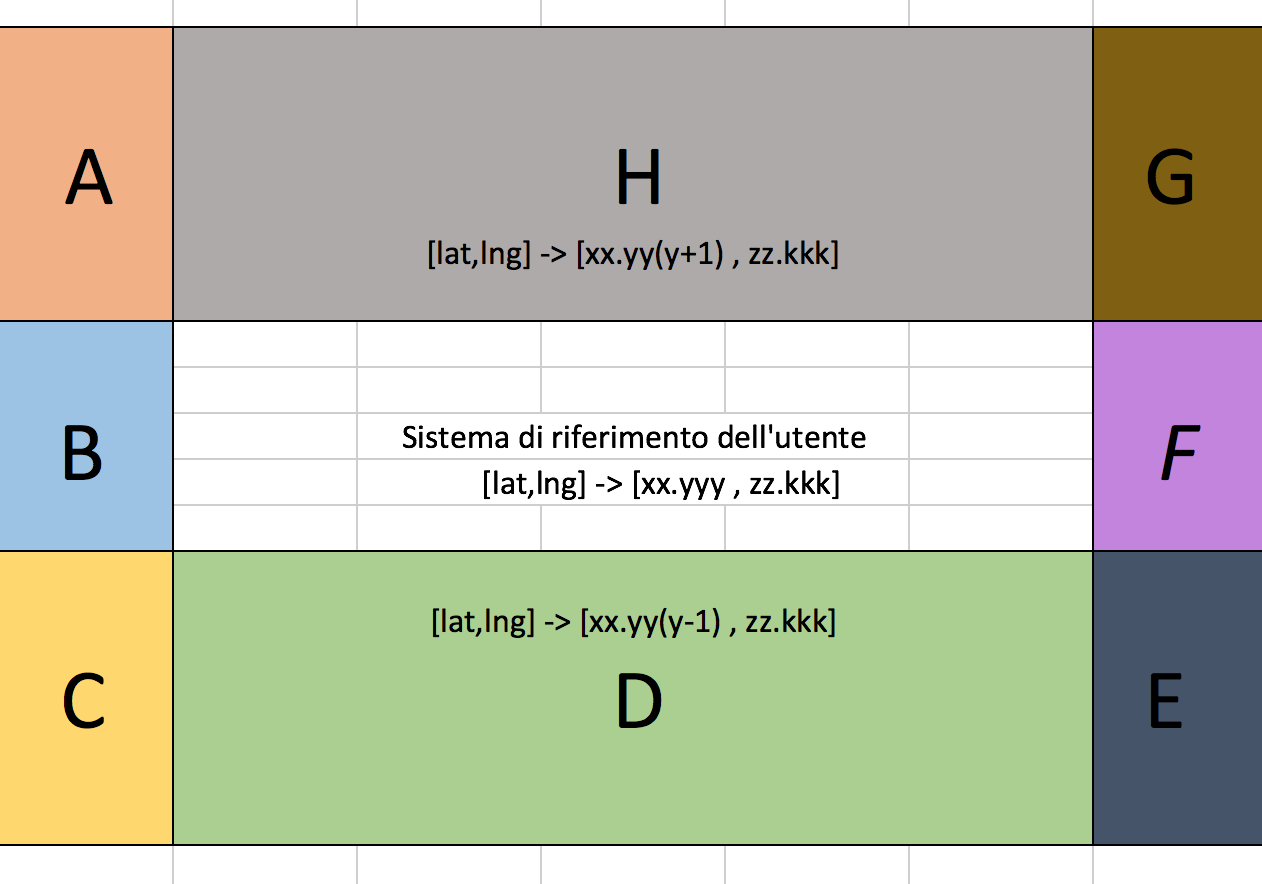
\includegraphics[scale=0.6]{Implementazione/sis1.png}
	\caption{Sistema di riferimento dell'utente}
	\label{fig:sis}
\end{figure}
\newpage
\item Le coordinate dell'utente (o dell'evento) vengono quindi troncate alla quarta cifra decimale che viene posta a zero, questo significa mappare tutte le persone, all'interno di un area rettangolare di  $88 mt^{2}$, nell'angolo in basso a sinistra dello stesso rettangolo (ndr Santiago de Chile si trova in direzione sud-ovest dall'Italia, da cui il nome dell'algoritmo). Di seguito un'immagine per chiarire meglio il funzionamento.

\begin{figure}[H]
	\centering
	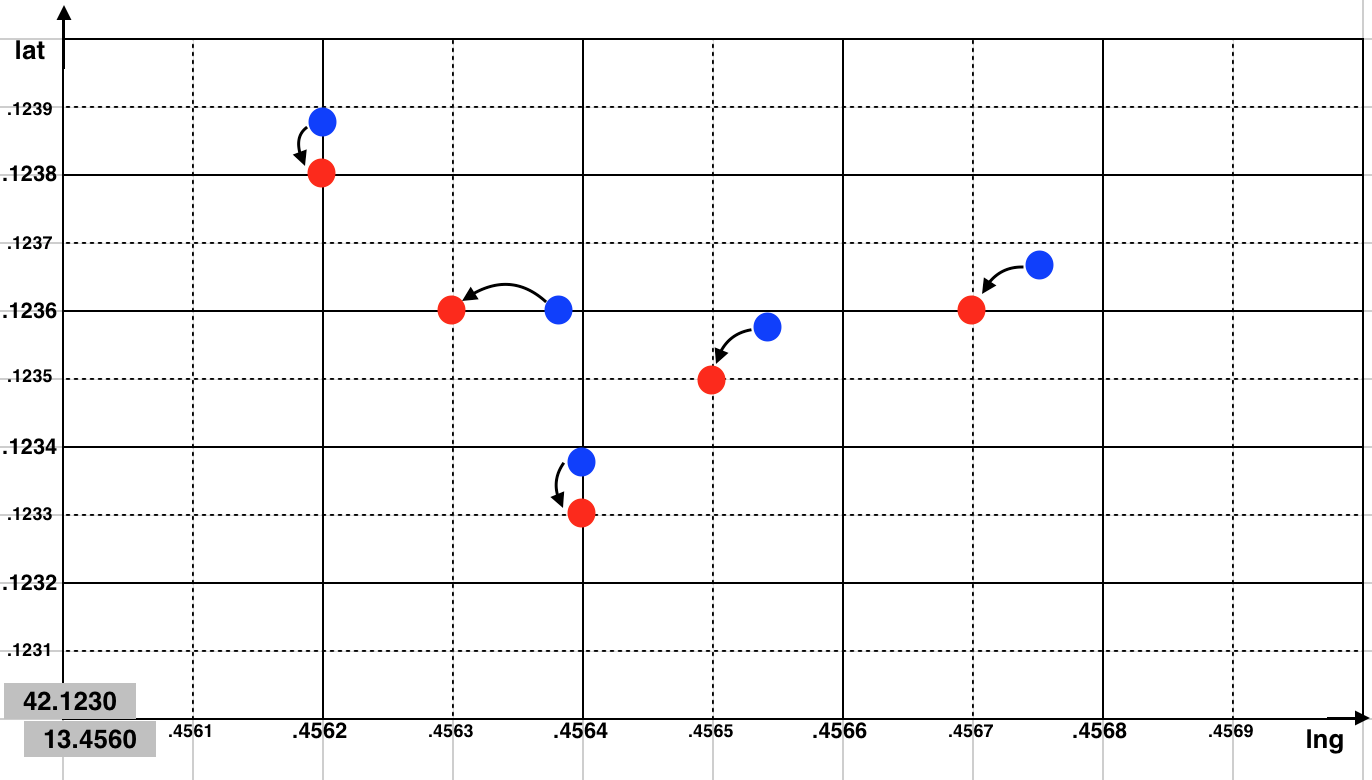
\includegraphics[scale=0.6]{Implementazione/mapping.png}
	\caption{Troncamento delle coordinate alla quarta cifra decimale posta a zero}
	\label{fig:mapping}
\end{figure}

I cerchi blu rappresentano le posizioni di diversi utenti, mentre i cerchi rossi rappresentato le posizioni dopo il troncamento. E' bene osservare che i punti sui confini in alto e a destra vengono mappati nella cella (o sistema per quelli ai confini) successiva.
\newpage
\item Le specifiche impongono celle di grandezza doppia rispetto a quelle ottenibili semplicemente troncando le coordinate alla quarta cifra decimale, questo vuol dire che quattro rettangoli di grandezza $(11*8)mt^{2}$ compongono una cella della nostra griglia; così facendo ogni sistema è composto da 25 celle, come possiamo vedere nella figura successiva.
\begin{figure}[H]
	\centering
	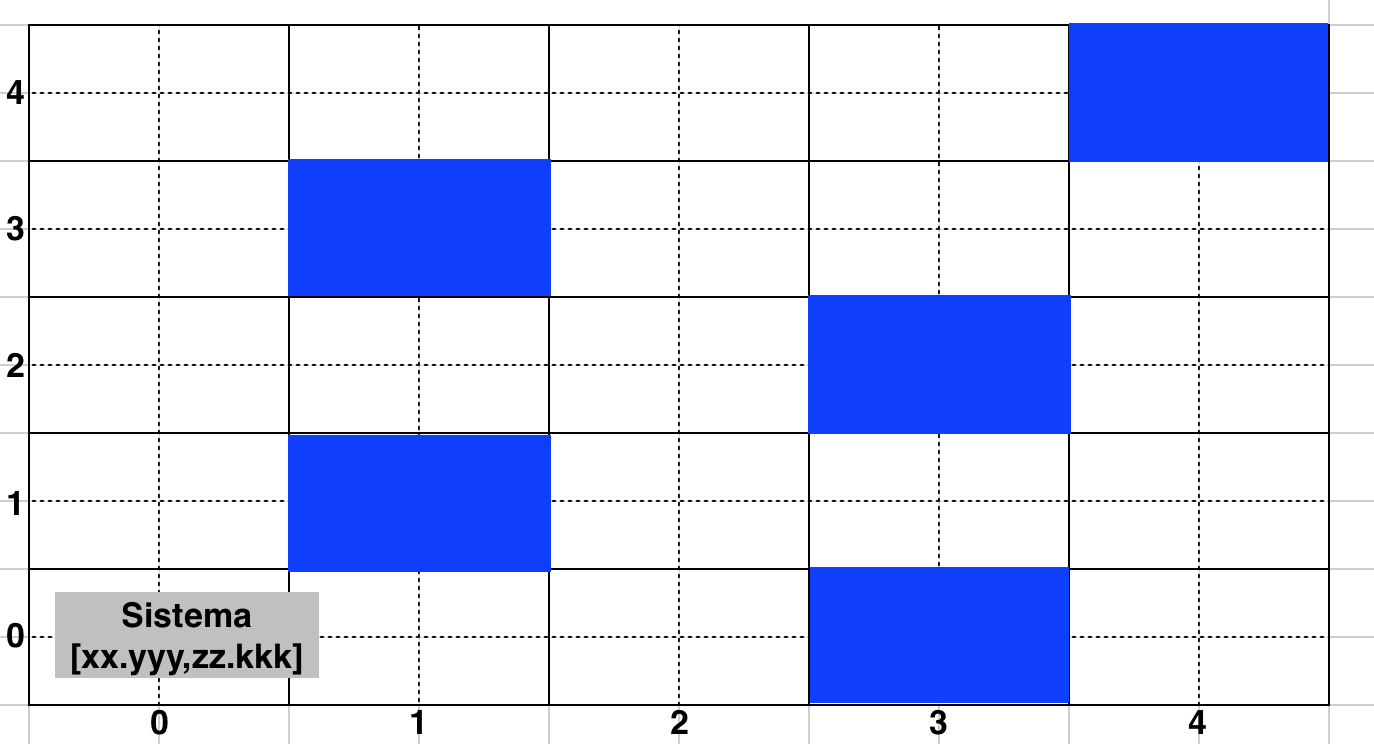
\includegraphics[scale=0.6]{Implementazione/celle.png}
	\caption{Alcune celle evidenziate in blu}
	\label{fig:celle}
\end{figure}
Quindi gli utenti/eventi sono \textbf{identificati senza ambiguità in tutto il globo} dalla seguente ennupla:
\begin{itemize}
\label{tupla}
\item Sistema di riferimento espresso in coordinate troncate alla terza cifra decimale $[xx.yyy,zz.kkk]$
\item Coppia di interi indicante il numero di cella all'interno del sistema  $[lat_y;lng_x]$
\end{itemize} 
\newpage
\item A questo punto bisogna ottenere la coppia di interi $[lat_y;lng_x]$, il sistema calcola la distanza dagli assi del sistema, dividendo in modulo per 22 quella con l'asse della latitudine e dividendo in modulo per 16 quella con l'asse longitudinale.
\begin{figure}[H]
	\centering
	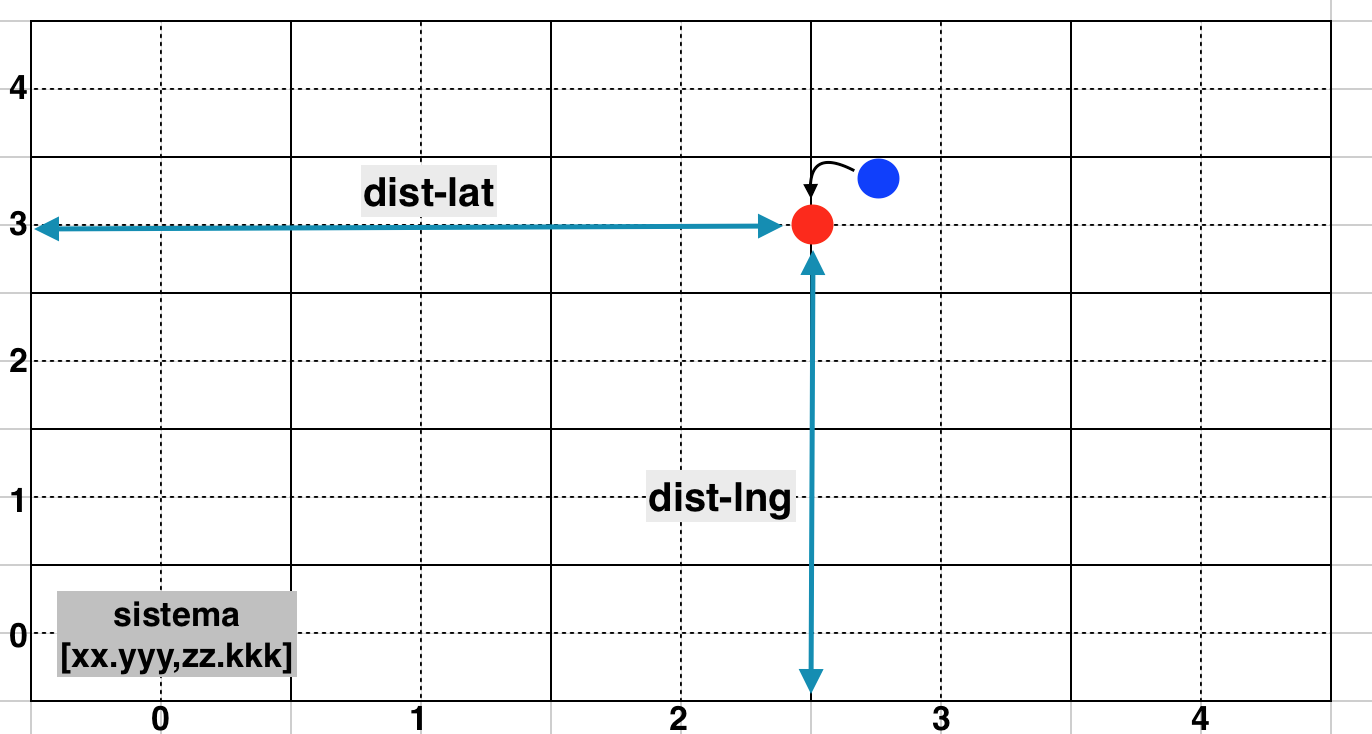
\includegraphics[scale=0.6]{Implementazione/dist.png}
	\caption{Proiezione delle distanze utilizzate per il calcolo della cella}
	\label{fig:dist}
\end{figure}
Poichè la distanza massima si ha in corrispondenza della cella $[4;4]$ ed equivale a $110 mt$, l'errore massimo di calcolo sarà pari a $33cm$. Questo è il motivo della scelta di un sistema con queste dimensioni, infatti troncando alla seconda cifra decimale avremo sistemi di $0.968km^{2}$ e un'errore di calcolo massimo pari a $3.3mt$, senza considerare l'aumento del costo computazionale richiesto. 
\end{enumerate}
\newpage

Il procedimento inverso consiste nella seguente formula:
\begin{equation}
\label{equazione}
 [xx.yyy;zz.kkk]+0.0001+([lat_y;lng_x]*0.0001*2)
\end{equation}
Così facendo tutti gli eventi/persone vengono mappati al centro delle varie celle, con un errore massimo dalla posizione reale (trascurando l'errore inevitabile del GPS) di $13mt$.
\begin{figure}[H]
	\centering
	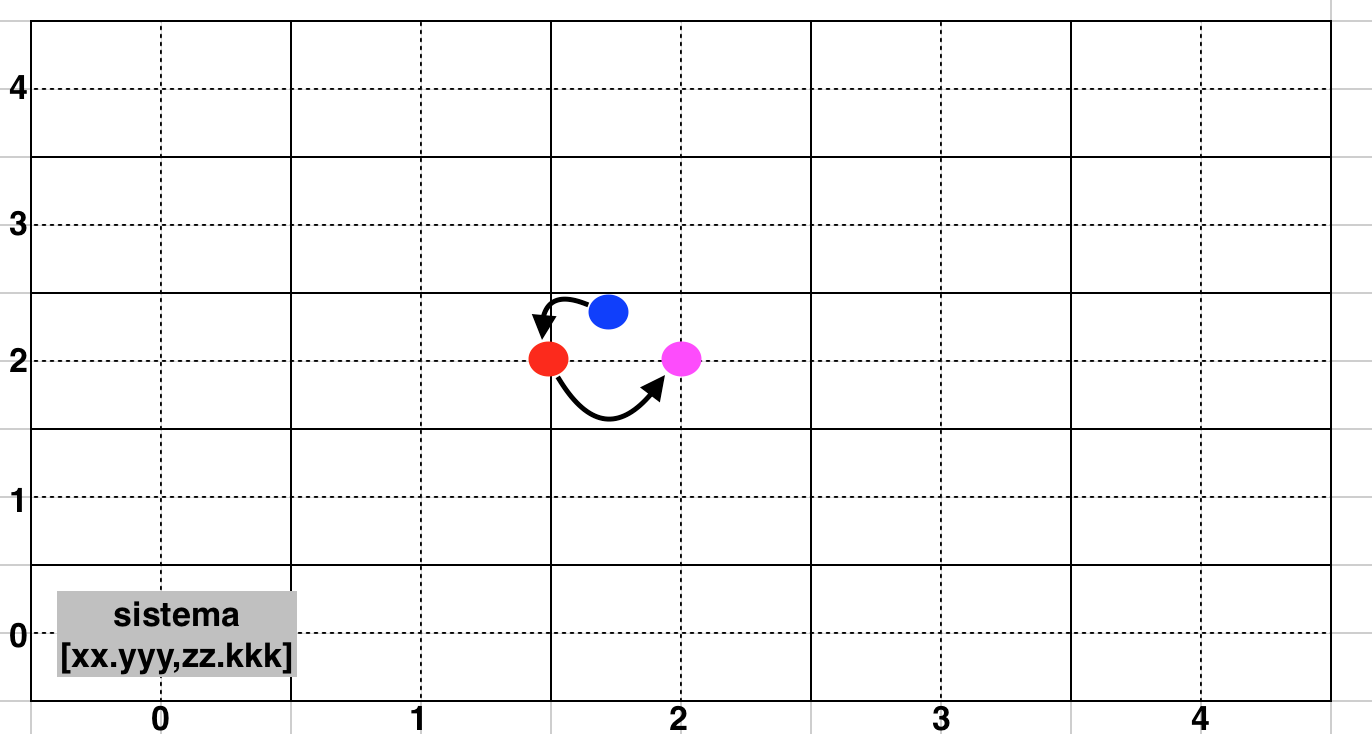
\includegraphics[scale=0.6]{Implementazione/final.png}
	\caption{Posizione ottenuta riconvertendo la tupla di dati vista nel passo \ref{tupla} dell'algoritmo }
	\label{fig:final}
\end{figure}
\newpage
\subsection{Il codice}
Vediamo quindi il codice \textit{Javascript} utilizzato per implementare l'algoritmo di Santiago. La prima funzione calcola il sistema e la posizione dell'evento o della persona all'interno di esso.
\begin{lstlisting} [language=JavaScript]

latLng->{lat:Number,lng:Number}

calcCell:function(latLng){
   var lat=latLng.lat;
   var lng=latLng.lng;
   var cut=Math.pow(10,4); 
  //coordinate origine del sistema
   var coordinates=L.latLng(Math.floor(lat*cut)/cut,Math.floor(lng*cut)/cut);  
  //coordinate perpendicolari lat e lng
   var perpendicular_lat=L.latLng(Math.floor(coordinates.lat*1000)/1000,coordinates.lng); 
   var perpendicular_lng=L.latLng(coordinates.lat,Math.floor(coordinates.lng*1000)/1000);  
 //richiama un metodo per il calcolo della distanza utilizzando l'algoritmo di Haversine
   var dist_lat=this.calcDist(coordinates,perpendicular_lat).haversine; 
   var dist_lng=this.calcDist(coordinates,perpendicular_lng).haversine;
   var dist={dist_lat,dist_lng};
//divisione in modulo per trovare la cella all'interno del sistema
   var cell_number_lat=Math.floor(dist_lat/22);
   var cell_number_lng=Math.floor(dist_lng/16);
   var cell={cell_number_lat,cell_number_lng};
   return ({zero:L.latLng(perpendicular_lat.lat,perpendicular_lng.lng),cell});
	},
\end{lstlisting}
\newpage

E ora il codice per l'equazione inversa (\ref{equazione}):
 \begin{lstlisting} [language=JavaScript]
 data-> {zero:{latLng},cell:{cell_number_lat(Number),cell_number_lng(Number)}}
 
 coordFromCell:function(data){

	 return L.latLng(data.zero.lat+0.0001+(data.cell.cell_number_lat*0.0001*2),data.zero.lng+0.0001+(data.cell.cell_number_lng*0.0001*2));
	 
	},
\end{lstlisting}
\newpage

\section{La struttura architetturale}
Come detto l'applicazione deve comunicare con un main-server, quindi l'architettura è quella classica delle applicazioni web, ovvero client-server.	 Tuttavia si è pensato di utilizzare anche il concetto di REST.\\
REST \cite{REST} definisce un insieme di principi architetturali per la progettazione di un sistema. Rappresenta uno stile architetturale, cioè non si riferisce ad un sistema concreto e ben definito né si tratta di uno standard stabilito da un organismo di standardizzazione. \\ 
Le risorse sono gli elementi fondamentali su cui si basano i Web Service RESTful, a differenza dei Web Service SOAP-oriented che sono basati sul concetto di chiamata remota. Per risorsa si intende un qualsiasi elemento oggetto di elaborazione. Per fare un parallelo con la programmazione ad oggetti possiamo dire che una risorsa può essere assimilata ad una istanza di una classe.\\
Il principio che stiamo analizzando stabilisce che ciascuna risorsa deve essere identificata univocamente. Essendo in ambito Web, il meccaniscmo più naturale per individuare una risorsa è dato dal concetto di URI. \\
\begin{figure}[H]
	\centering
	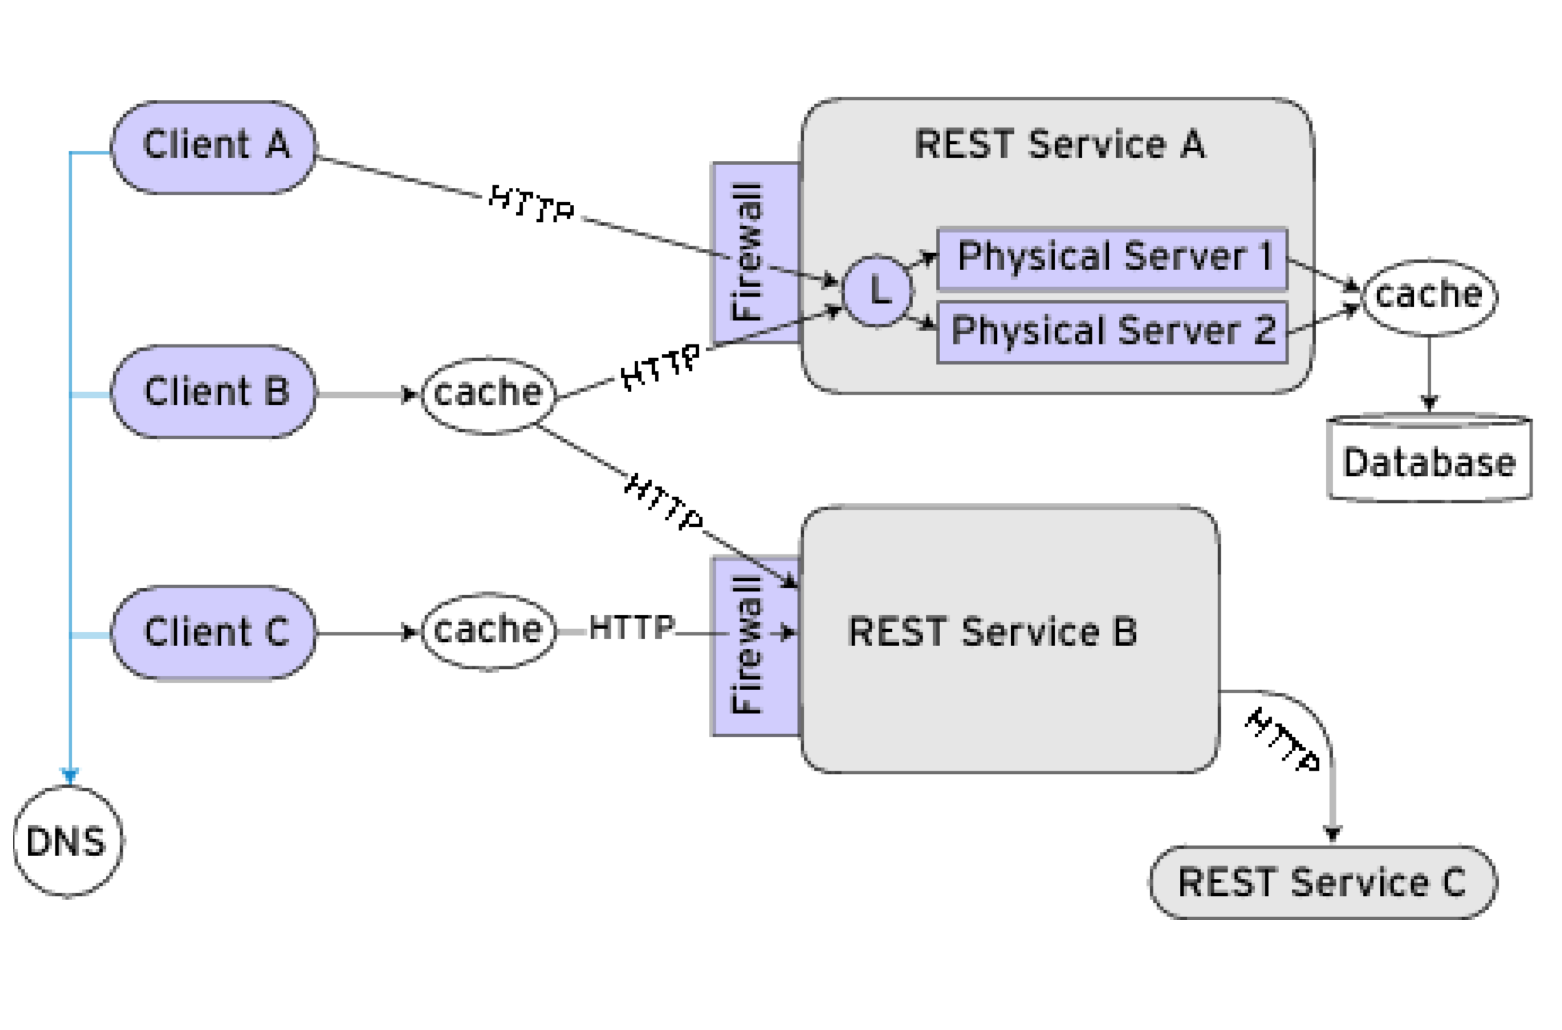
\includegraphics[scale=0.5]{Implementazione/rest.png}
	\caption{Rappresentazione semplificata dell'architettura }
	\label{fig:rest}
\end{figure}

Così facendo, non si deve implementare un metodo del tipo "\textit{getDati(idutente)}", ma basterà eseguire una chiamata HTTP con metodo GET alla risorsa \\
"\textit{http://www.myapp.com/dati/idutente}". Questo approccio permette quindi di definire un'interfaccia tra il client e il server, rendendo quest'ultimo più scalabile. 
La realizzazione del server non è argomento di questa tesi, tuttavia è necessario definire la struttura dei dati trasmessi e ricevuti dall'applicazione, in modo tale che in futuro il progettista del server possa implementare il REST service come meglio crede purché rispetti il formato dei dati stabilito. \\
Di seguito i sequence diagram relativi alla richiesta e la trasmissione di informazioni tra il client e il server, per ognuni pacchetto verrà mostrato il formato stabilito.\\ \\
 \textbf{Richiesta dei propri FOI e POI:} In questa fase l'applicazione deve ricevere i dati sui POI e i FOI dell'utente. Il formato della risorsa dipenderà dal successo o meno della richiesta. Il pacchetto ErrorFP è lo stesso generato dall'applicazione in caso di rete assente. \\
 \begin{figure}[H]
	\centering
	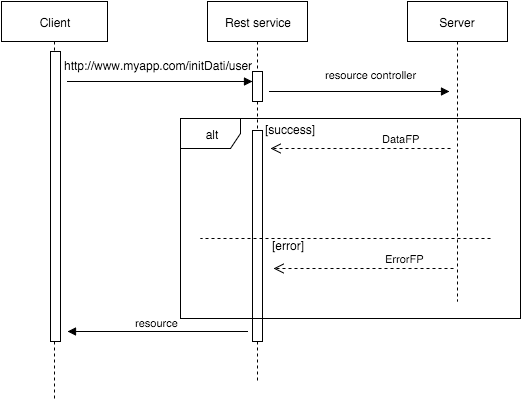
\includegraphics[scale=0.7]{Implementazione/foipois.png}
	\caption{Rappresentazione della sequenza di azioni per la richiesta dei propri FOI e POI }
	\label{fig:rest}
\end{figure}
\begin{itemize}
\item \textit{GET http://www.myapp.com/initDati/user}, è l'URI della risorsa contenente le informazioni sui POI e i FOI dell'utente. Il parametro \textit{user} serve per identificare l'utente che sta facendo la richiesta.
\item \textit{DataFP}, in caso di successo la resource è nel seguente formato:\\
\begin{lstlisting} [language=JavaScript]
{
poi:[
		{
			nome: String,
			foto: String,
			emergency: String,
			icon: String,
			number: Integer,
			ultimo_ora: String,
			ultimo_data: String,
			position: 
			{
			     zero:{
			              lat: Number,
			              lng: Number
			              },
			     cell:{
			              cell_number_lat: Number,
			              cell_number_lng: Number
			            }
			}
			
	  },
	  .
	  .
	  .
	],
foi:[
	  {
			nome: String,
			foto: String,
			stato: String,
			cod_emergency: Integer,
			ora_stato: String,
			data_stato: String,
			distanza: Number,
			dispositivo: String,
			ora_dispositivo: String,
			position: 
			{
			     zero:{
			              lat: Number,
			              lng: Number
			              },
			     cell:{
			              cell_number_lat: Number,
			              cell_number_lng: Number
			            }
			}
	  },
	  .
	  .
	  .
	]
}
\end{lstlisting}
\item \textit{ErrorFP}, in caso di errore la resource è semplicemente una stringa:\\
\begin{lstlisting} [language=JavaScript]
{
  error: String
}
\end{lstlisting}
\end{itemize}
\newpage
 \textbf{Aggiornamento status:} di seguito si illustrano le azioni legate all'aggiornamento dello status di un'utente (client A). La sequenza si compone di una prima fase, nella quale l'utente chiede al server di modificare la risorsa corrispondente al suo status, è una seconda fase nella quale un altro utente (client B), che ha tra i suoi FOI il precedente, richiede al server l'aggiornamento dei dati (l'algoritmo legato ai tempi e i modi di aggiornamento dei propri dati non è stato sviluppato, andrebbe fatto tenendo conto del contesto e dello stato della rete).\\
 \begin{figure}[H]
	\centering
	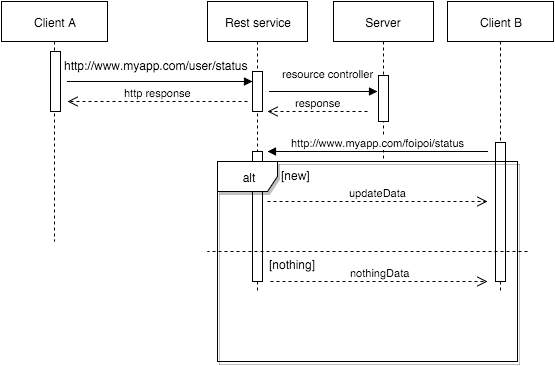
\includegraphics[scale=0.8]{Implementazione/updateStatus.png}
	\caption{Rappresentazione semplificata dell'architettura }
	\label{fig:rest}
\end{figure}
\begin{itemize}
\item \textit{PUT http://www.myapp.com/iduser/status}, è l'URI della risorsa contenente le informazioni sull'utente "\textit{user}". Questo parametro serve infatti ad identificarlo, mentre lo status è nel seguente formato:\\
\begin{lstlisting} [language=JavaScript]
{
 stato: String,
 cod_emergency: Integer,
 ora_stato: String,
 data_stato: String,
  
}
\end{lstlisting}
Per il successo dell'operazione è sufficiente verificare la response http del server direttamente nell'applicazione.
\item \textit{GET http://www.myapp.com/iduser/foi/status},è l'URI della risorsa contentente tutte le informazioni dei FOI di un relativo utente (parametro \textit{iduser} per identificare l'utente che richiede la risorsa).
\item \textit{updateData}, 
\end{itemize}